% Created 2020-09-30 Wed 15:22
% Intended LaTeX compiler: pdflatex
\documentclass[10pt,t]{beamer}
\usepackage[utf8]{inputenc}
\usepackage{graphicx}
\usepackage{grffile}
\usepackage{longtable}
\usepackage{wrapfig}
\usepackage{rotating}
\usepackage{textcomp}
\usepackage{amssymb}
\usepackage{capt-of}
\usepackage{hyperref}
\usetheme{default}
%
\usepackage[font=small,labelfont=bf]{caption} % Required for specifying captions
\usepackage{subcaption}
%
\author{C. L. Hepplewhite}
\date{\today}
\title{\large CHIRP Radiance Corrections/Offsets Connecting AIRS, SNPP, JPSS-1, and IASI}
\subtitle{\footnotesize{AIRS Virtual Science Team Meeting}}
\date{\vspace{0.1in}\footnotesize{October 2020 \vfill}}
\author{C. L. Hepplewhite\inst{1,2}, L. Larrabee Strow\inst{1,2}, and Howard Motteler\inst{2} }
\institute[UMBC]{\inst{1} UMBC Physics Dept. \and \inst{2}UMBC JCET}
\input beamer_setup
\metroset{titleformat title=allcaps}
\setbeamertemplate{frame footer}{UMBC Atmospheric Spectroscopy Lab}
\begin{document}

\maketitle

\begin{frame}{Summary}
\begin{itemize}
  \item What is CHIRP
  \item What are radiance offsets for connecting AIRS, CrIS and IASI.
  \item Data and methods used to derive the radiance offsets.
  \item Results and Discussion.
  \item Integration of offsets into the CHIRP L1C.
    
\end{itemize}

\end{frame}
% -----------------------------------------------------
\begin{frame}{What is CHIRP}

  \begin{itemize}
  \item Climate Hyperspectral InfraRed Product is derived sequentially from
    multiple similar sensors in low earth orbit to create an on-going radiance
    record from the start of AIRS to the present.
  \item CHIRP data are available as level 1 calibrated, geolocated granules.
    (Details are provided in the accompanying presentation and on-line documentation).
  \item Current working version of CHIRP connects AIRS to CrIS from SNPP and JPSS1.
  \item and has the spectral resolution of CrIS in medium resolution, equivalent to:
    0.8/0.6/0.4 cm interferometric OPD (LW/MW/SW).
  \item Of concern in this work is that the radiometric calibration is stable (has
    a fixed relationship to absolute truth, known to be 'small'), and there is no
    radiometric change in CHIRP going from one parent (AIRS) to another (CrIS).
  \end{itemize}
  

\end{frame}
% -----------------------------------------------------
\begin{frame}{What are the Radiance Offsets}

  \begin{itemize}
  \item The radiance offset betwen two sensors is the radiometric calibration
    difference observed when they are both measuring the same scene at the same time.
  \item In principle, radiometric calibration offsets could be a function of time and
    brightness temperature and may be non-linear.
  \item Ideally the best result would be to cross-calibrate the sensors against a primary
    standard black body - instead must use data available during the missions.
  \item Fortunately there is a lot of mission overlap between AIRS, CrIS and IASI
    (more details to follow).
  \item CHIRP V1 derived from AIRS or J1-CrIS have BT bias offsets applied to convert them to the NPP-CrIS radiometric calibration.

  \end{itemize}

\end{frame}

% -----------------------------------------------------
\begin{frame}{Data and Methods}

  \begin{itemize}
    \item Data used: SNOs and global random statistical samples.
    \item Periods analyzed include all available mission overlaps.
    \item Available mission overlaps for
      \begin{itemize}
      \item AIRS:NPP from Apr 2012 to present (Dec 2015 at FSR).
      \item AIRS:J1 from Jan 2018 to present.
      \item NPP:J1 from Jan 2018 to present.
      \item AIRS:IASI1 from May 2007 to present.
      \item NPP and J1:IASI1. (Note: SNOs are not available for NPP:J1).
      \end{itemize}
      
    \item The transition date for parent AIRS to parent CrIS SNPP is 01-Sep-2016.
    \item The switch to JPSS1 is proposed 01-Sep-2018 to avoid the 2019 SNPP CrIS
      shutdown.

  \end{itemize}
\end{frame}

% -----------------------------------------------------
\begin{frame}{Data and Methods 2}

  \begin{itemize}
  \item Two Sources of intercalibration data are available: SNOs and global random samples.
  \item SNOs have the advantage of being matched pairs of observations, but are spatially less uniformly distributed than global random.
    \begin{itemize}
    \item AIRS:CrIS SNOs are global but weighted to high latitudes,
    \item IASI:CrIS SNOs are restricted to a very narrow latitude band near 70-deg.
    \end{itemize}
  \item both SNOs and random samples can be used for trending and for scene dependencies.
  \item In the following bias plots the mission overlap period March.2018 to Feb.2019 (incl.) is used.
    
  \end{itemize}

\end{frame}

% ----------------------------------------------------
\begin{frame}{Data and Methods 3}
  
\begin{figure}
\centering
\begin{subfigure}{.5\textwidth}
  \centering
  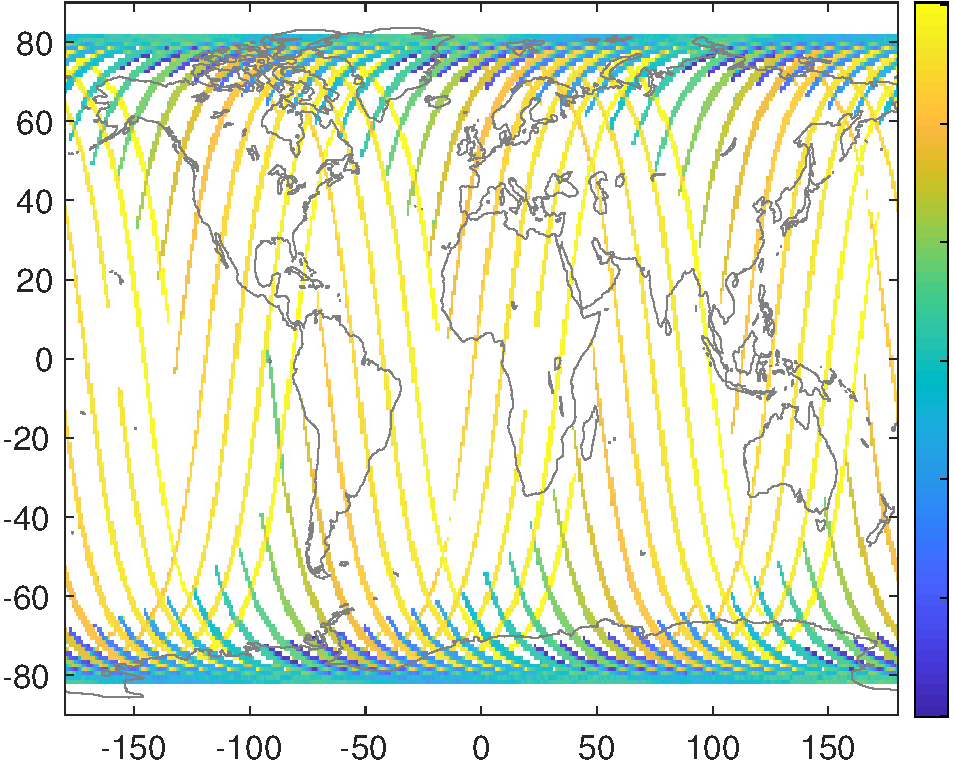
\includegraphics[width=.4\linewidth]{ac_global_delay_map.pdf}
  \caption{A subfigure}
  \label{fig:sub1}
\end{subfigure}%
\begin{subfigure}{.5\textwidth}
  \centering
  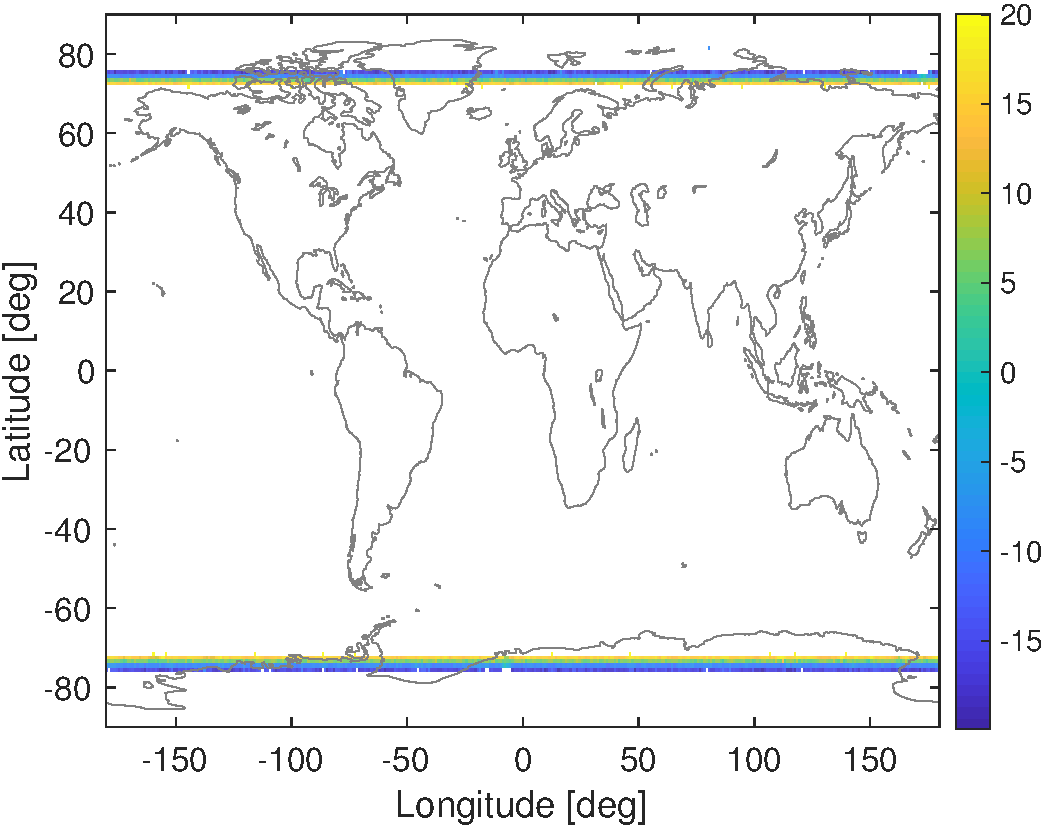
\includegraphics[width=.4\linewidth]{ai_global_delay_map.pdf}
  \caption{A subfigure}
  \label{fig:sub2}
\end{subfigure}
\caption{A figure with two subfigures}
\label{fig:test}
\end{figure}

\end{frame}

% -----------------------------------------------------
\begin{frame}{Results 1. AIRS:NPP bias versus AIRS modules}

\vspace{-0.1in}
  \begin{center}
    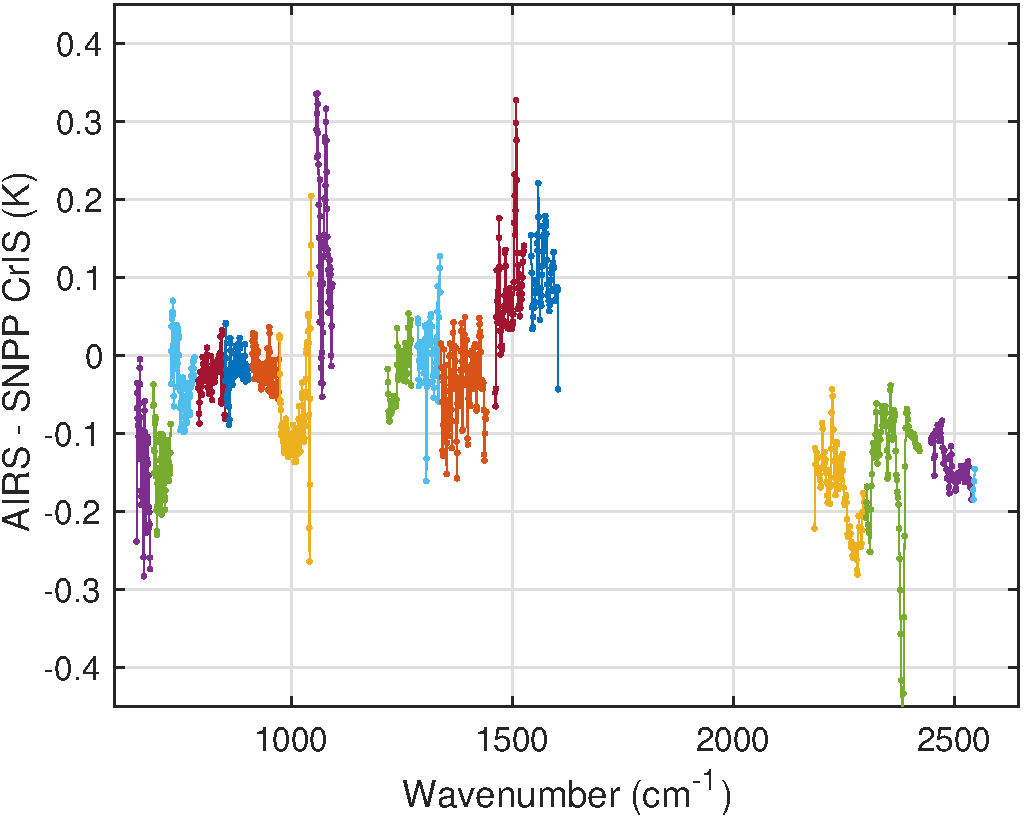
\includegraphics[width=0.7\linewidth]{./Strow/airs_minus_cris_airs_array_colors.pdf}
    \captionof{figure}{AIRS bias relative to SNPP from global statistics. Colors denote AIRS detector modules.}
\end{center}
  \end{frame}

% -----------------------------------------------------
\begin{frame}{Results 2. AIRS:NPP bias with fill and bad channels}

\vspace{-0.1in}
  \begin{center}
%    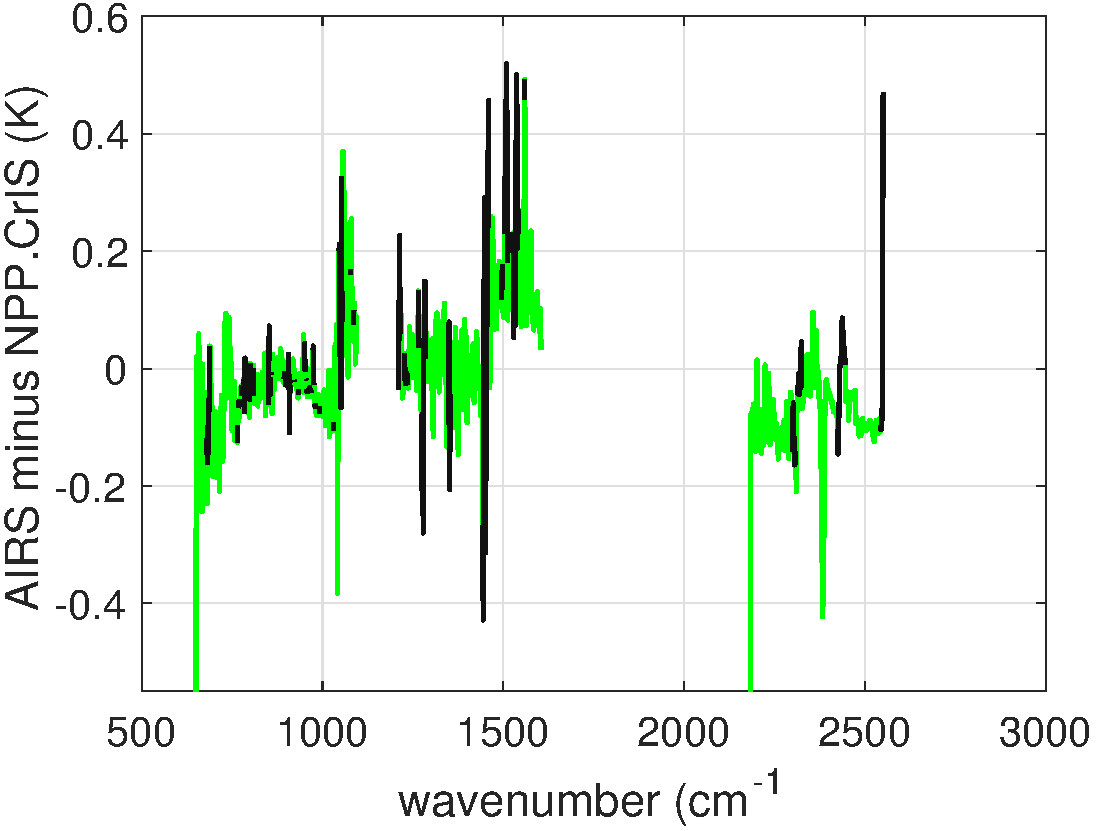
\includegraphics[width=0.6\linewidth]{./Figs/2018_airs_npp_ac1_stats_bias_wbad_fill.pdf}
   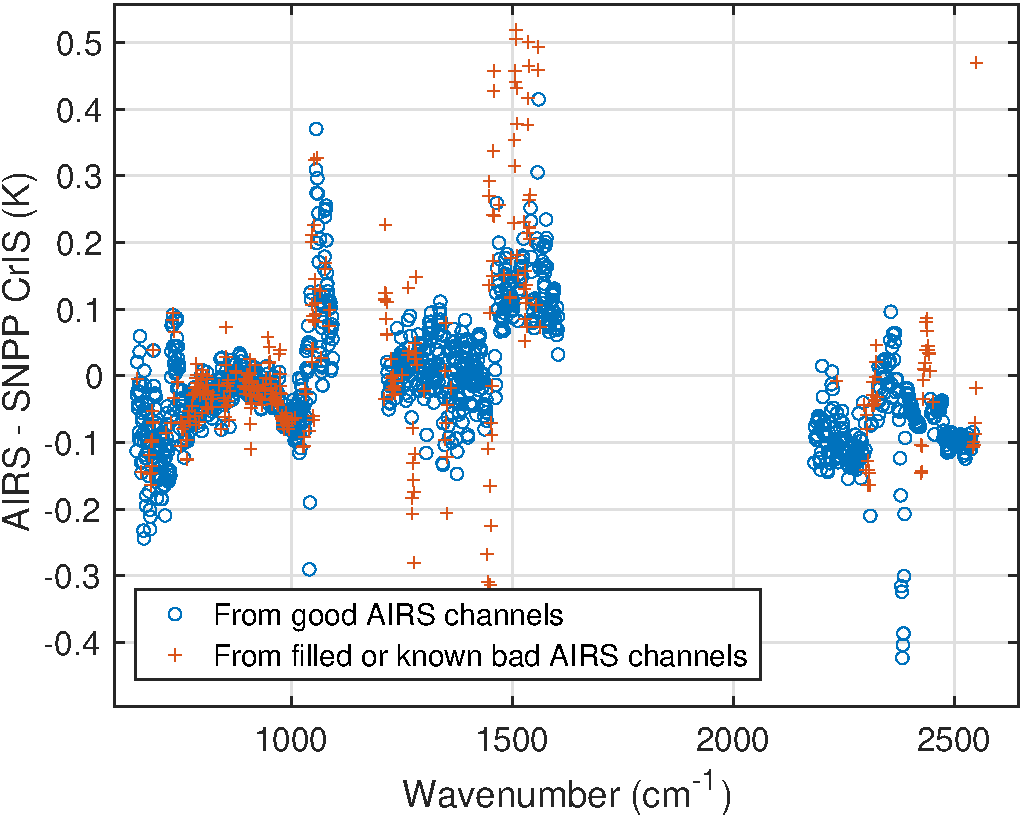
\includegraphics[width=0.7\linewidth]{./Strow/lls_2018_airs_npp_ac1_stats_bias_wbad_fill_v2.pdf}
    \captionof{figure}{AIRS bias relative to SNPP from global statistics. Showing parent bad or fill channels (total of 356).}
  \end{center}
    
\end{frame}

% -----------------------------------------------------
\begin{frame}{Results 3. AIRS:NPP and AIRS:J1 bias}

\vspace{-0.1in}
\begin{block}{}
  \begin{center}
    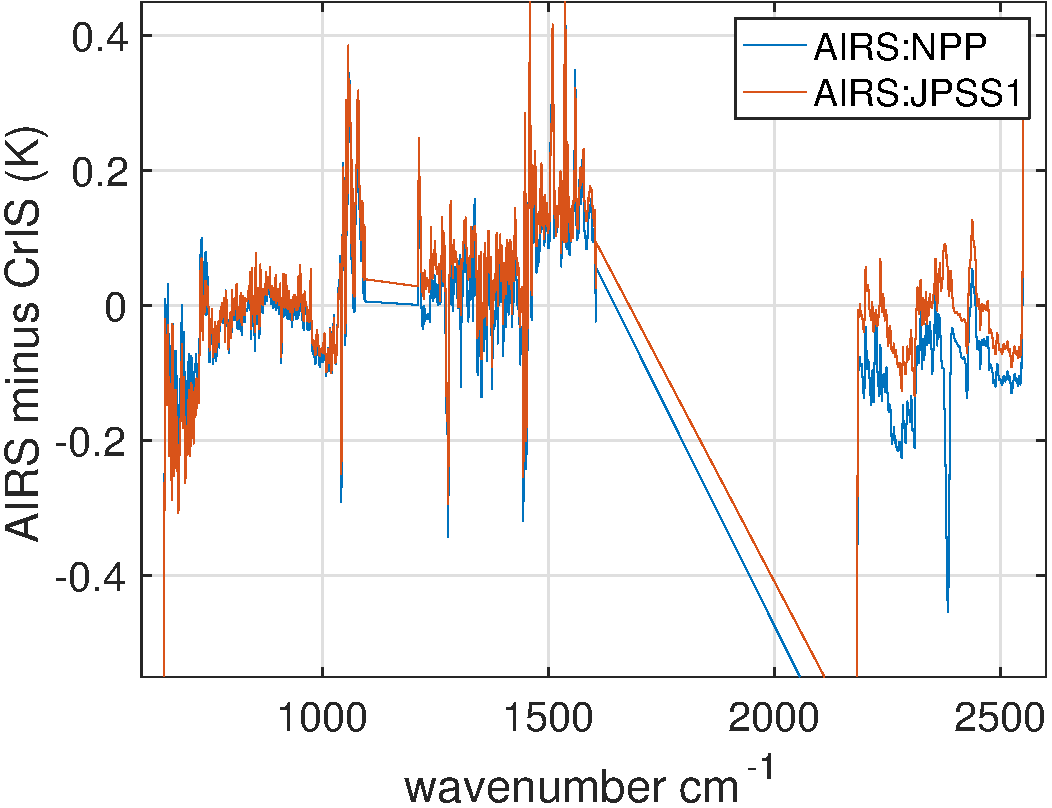
\includegraphics[width=0.6\linewidth]{./Figs/2018d060_2019d059_ac1_ac2_sno_mean_bias.pdf}
    \captionof{figure}{CHIRP channels. AIRS bias relative to SNPP and J1 from SNO. One year of data. Double difference can be used for NPP:J1 bias.}
  \end{center}
\end{block}
    
\end{frame}

% -----------------------------------------------------
\begin{frame}{Results 4. AIRS:NPP bias From Stats and SNOs}

  \begin{center}
    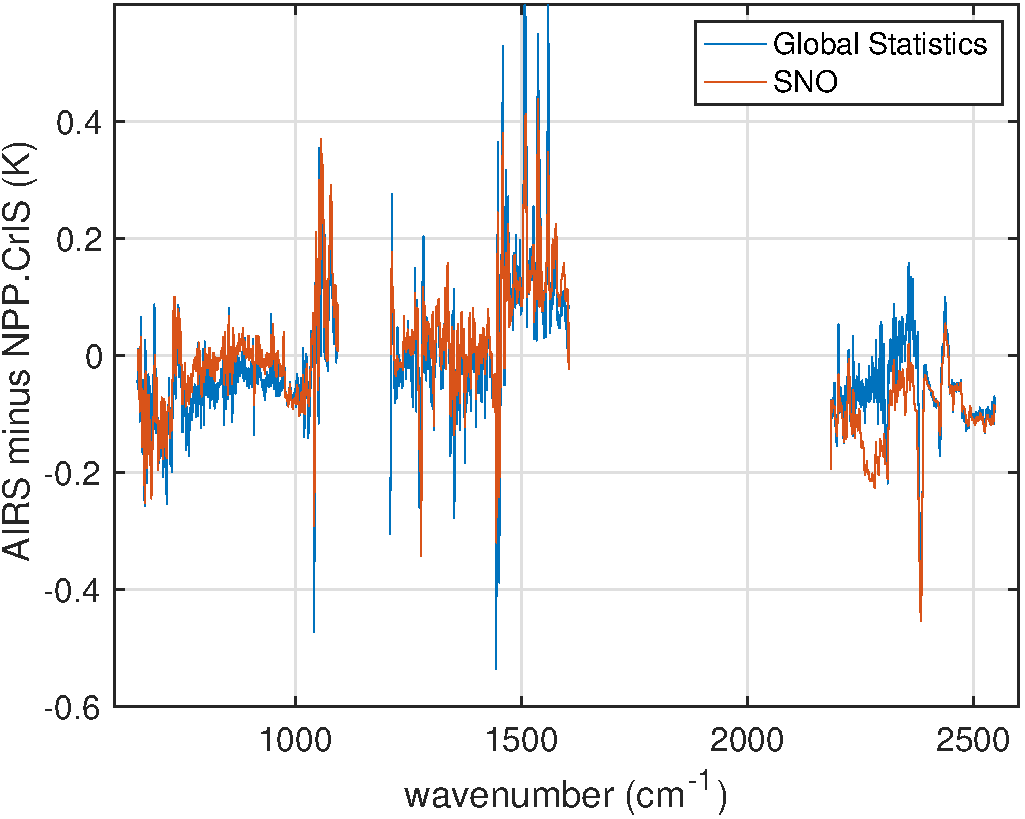
\includegraphics[width=0.65\linewidth]{./Figs/2018d060_2019d059_airs_npp_ac1_bias_stats_sno_v2.pdf}
    \captionof{figure}{AIRS bias relative to SNPP from SNO and global stats.  Good agreement, \sim0.03K.}
  \end{center}
    
\end{frame}

% -----------------------------------------------------
\begin{frame}{Results 5. J1:NPP bias}

\vspace{-0.1in}
  \begin{center}
    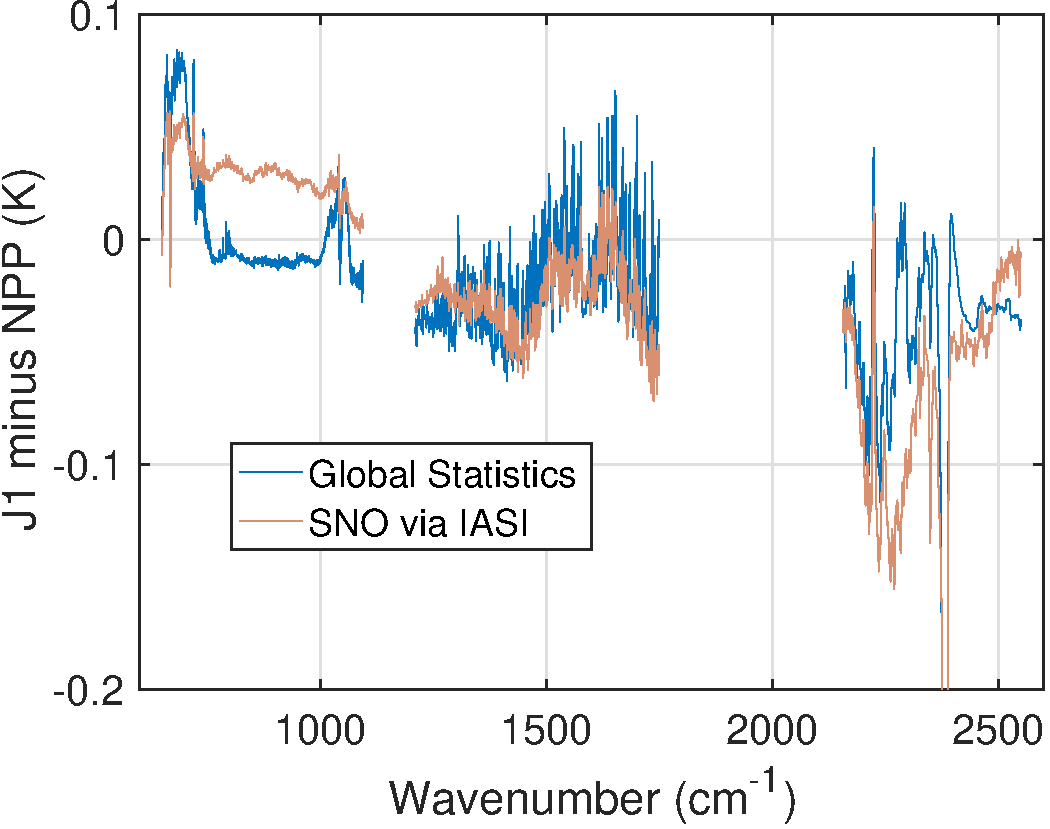
\includegraphics[width=0.7\linewidth]{./Figs/2018_jn_ic1_ic2_stats_sno_bias_v2.pdf}
    \captionof{figure}{CHIRP channels. CrIS bias from JPSS-1 relative to SNPP from SNO using IASI.1 as cross reference and from global random stats.}
  \end{center}
    
\end{frame}

% -----------------------------------------------------
\begin{frame}{Results 6. Bias variation with irradiance.}

  \begin{center}
    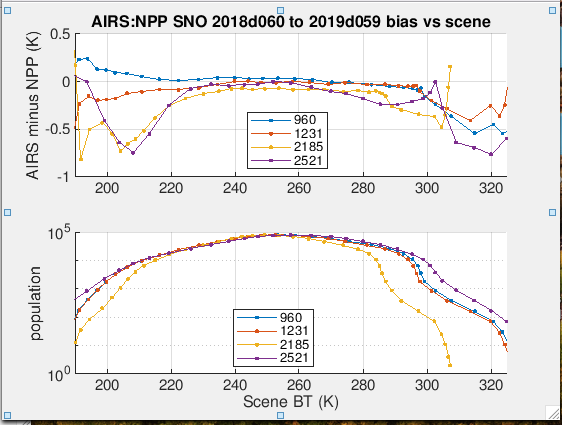
\includegraphics[width=0.6\linewidth]{./Figs/plot1.png}
    \captionof{figure}{Four CHIRP channels. Bias variation with irradiance from SNO.}
  \end{center}

  
\end{frame}

% -----------------------------------------------------
%\begin{frame}{Results 7. Sample of bias stability.}
%
%  \begin{center}
%    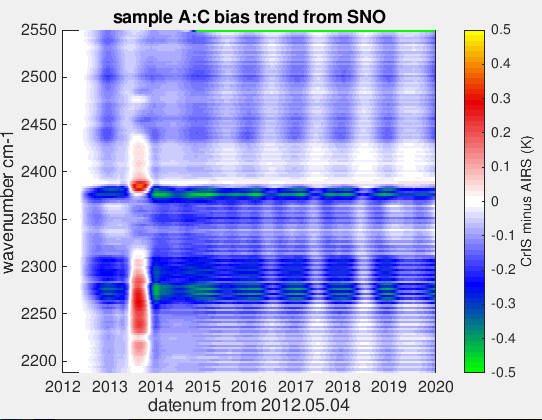
\includegraphics[width=0.6\linewidth]{./Figs/plot6.png}
%    \captionof{figure}{CHIRP short wave channels. Bias variation from AIRS:CrIS SNOs. Note %residual variation mostly from AIRS solar beta- dependent variation, and 2013 jump to be %investigate further.}
%  \end{center}
%    
%\end{frame}
%
% -----------------------------------------------------
\begin{frame}{Summary, Conclusions and Future Work}

  \begin{itemize}
  \item Radiometric offset vectors have been determined to tie CHIRP derived from AIRS to NPP:CrIS and J1:CrIS.
  \item The current CHIRP product includes a single valued vector for every channel.
  \item The bias has been found to be stable over the period of interest, which is 2016 to 2019.
  \item The dependency of bias on irradiance has been investigated, and some examples have been illustrated.
  \item Future work includes validation of the CHIRP product with particular attention to equivalence of trends of parents sensor.
    
  \end{itemize}
  

\end{frame}

% -----------------------------------------------------
%\begin{frame}[label={sec:org409cb32}]{Two}
%\vspace{-0.6in}
%\begin{columns}
%\begin{column}{0.55\columnwidth}
%\begin{block}{}
%\begin{center}
%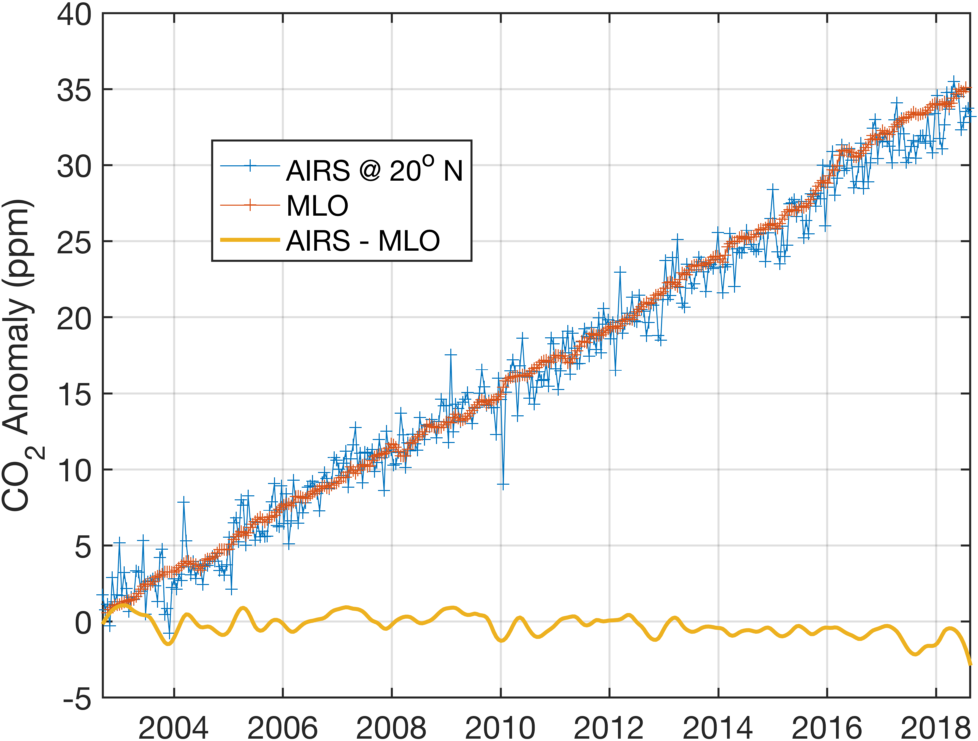
\includegraphics[width=\linewidth]{./Figs/airs_vs_mlo_co2_anom_jun24.png}
%\end{center}
%\end{block}
%\end{column}
%\end{columns}
%\end{frame}
% -----------------------------------------------------

% \begin{center}
% 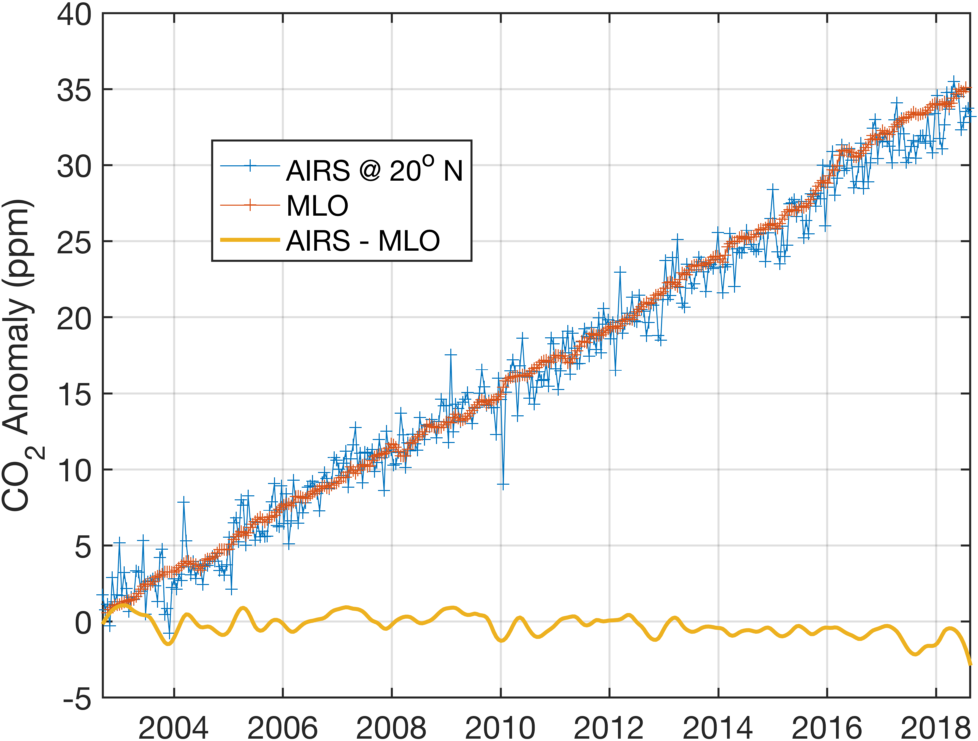
\includegraphics[width=0.8\linewidth]{./Figs/airs_vs_mlo_co2_anom_jun24.png}
% \end{center}

\end{document}

%%% Local Variables:
%%% mode: latex
%%% TeX-master: t
%%% End:
